\chapter{Unmarked Populations}
\markboth{Unmarked Populations}{}
\label{chapt.scr-unmarked}

\vspace{0.3cm}

Traditional capture-recapture models share the fundamental
assumption that each individual in a population can be uniquely
identified when captured. Often, this can be accomplished
by marking individuals with color bands, ear tags, or some other
artificial mark that subsequently can be read in the field. For other
species, such as tigers (\textit{Panthera tigris}) or marbled
salamanders (\textit{Ambystoma opacum}), individuals can be identified
using only their natural markings. However, many species
do not possess adequate natural markings and are
difficult to capture, making it impractical to use standard
capture-recapture techniques.

Estimating density when individuals are unmarked can be accomplished
using a variety of alternatives to capture-recapture, such as distance
sampling \citep{buckland_etal:2001} and $N$-mixture models
\citep{royle:2004biom}. These methods can be
very effective when their assumptions are met, but
when it is not possible to obtain accurate distance data, or when
movement complicates the use of fixed-area plots,
these methods may yield biased estimates of density
\citep{chandler_etal:2011}. Furthermore, some species are so rare and
cryptic that it is nearly impossible to collect enough data using
traditional survey methods.

In this chapter, we investigate spatially explicit alternatives for estimating density
of unmarked populations, and we highlight the work of
\citet{chandler_royle:2012} who demonstrated that the ``individual
recognition'' assumption of traditional capture-recapture models is not a
requirement of spatial capture-recapture models. They showed that,
under certain conditions, spatially correlated count
data are sufficient for making inference about animal distribution and
density even when no individuals are marked.
The \citet{chandler_royle:2012} ``spatial count model'' (hereafter the SC
model) requires neither distance data nor fixed area plots. Instead,
the observed data are trap- and occasion-specific counts, which
are modeled as a reduced-information summary of the \textit{latent}
encounter histories. Because the model is formulated in terms of the
data we wish we had, i.e. the typical encounter history data observed
in standard capture-recapture studies of marked animals, the SC model
is just a SCR model with a single extension to account for the fact
that the encounter history data are unobserved. However, this results
in a drastically different model than the models typically used for
count data in ecology because the SC model is parameterized in terms of
individuals, and specifically, their locations relative to the
sampling device.

The ability to fit SCR models to data from unmarked populations has
important implications. For one, it means that SCR models can
be applied to data collected using methods like points counts in which
observers record simple counts of animals at an array of survey
locations. The model can also be fitted to camera trapping data collected on
unmarked animals, representing one of the first formal method for estimating
density from such data \citep[but see][]{rowcliffe_etal:2008}.
So, is the SC model a free lunch? At face value, it sounds as though it
allows for estimation of all the quantities of interest in standard
capture-recapture studies, but with very little
data. But of course the answer is no -- lunch is still not free because
with this model come new assumptions, and as was demonstrated by
\citet{chandler_royle:2012}, even with ``perfect'' data, parameter estimates
will typically not be very precise. This should not be surprising
given that we are asking so much from simple count data.

The real value of the SC model is two-fold. First, it demonstrates
an important theoretical result, namely that spatial correlation in
count data carries information about density and distribution; a
result that stands in stark contrast to a prevailing view of
spatial correlation as a nuisance to be avoided or modeled out of unsightly
residual plots. The second reason why this model is important is that
it provides the basis for numerous model extensions that \textit{can}
yield precise density estimates. We will discuss some of
these possibilities in this chapter, but perhaps the most useful
extension -- accommodating data from both marked and unmarked
individuals -- is treated separately in the next chapter. Here, we focus
on situations in which all individuals are unmarked, and
we begin by presenting the most basic formulation of the model. Then we proceed, by
way of a few examples, to consider extensions of the model in which
ancillary information can be used to increase precision.

\section{Existing Models for Inference About Density in Unmarked Populations}
\label{Sect.existing-unmarked}
When capture-recapture methods are not a viable option, ecologists
often collect simple count data or even binary detection/non-detection
data. These data are often treated as an index of abundance or occurrence
and are analyzed using generalized linear models such as
Poisson regression or logistic regression, perhaps with random
effects \citep{zuur_etal:2009}. However, index methods cannot be used
to make unbiased inferences about abundance or occurrence unless
strong assumptions about constant detection probability are valid
\citep{williams_etal:2002,sollmann_etal:2013bioc}. In particular,
index methods can be highly misleading when covariates affect both the
ecological process of interest and the observation process. A classic
example is given by \citet{bibby_buckland:1987} who found that songbird detection
probability was negatively related to vegetation height, whereas
density was positively associated with vegetation height in restocked
conifer plantations. This intuitive phenomenon has been
demonstrated repeatedly \citep{kery:2008,sillett_etal:2012} and has led to the
development of a vast number of models to estimate population size and
occurrence probability when individuals are unmarked and detected
imperfectly
\citep{buckland_etal:2001,williams_etal:2002,mackenzie_etal:2006,royle_dorazio:2008}.
A review of these models is beyond the scope of this
chapter, but we mention a few deficiencies of existing methods
that warrant the exploration of alternatives for robust inference when
standard capture-recapture methods do not apply.

Distance sampling \citep{buckland_etal:2001,buckland_etal:2004book}, which we briefly
introduced in Chapter~\ref{chapt.closed},
is perhaps the most widely used method for
estimating population density when individuals are unmarked and
detection probability is less than one. This class of methods is known
to work impeccably when estimating the number of stakes in a field or
the number of duck nests in a wetland. Distance sampling can also work very well in
more interesting situations, and it is an extremely powerful method when
the assumptions can be met. However, the assumptions that distance
data can be recorded without error and that animals are distributed
randomly with respect to the transect can be easily violated by
common processes such as animal movement and measurement
error. Although numerous methods have been proposed to
relax some of these assumptions
\citep{royle_etal:2004, borchers_etal:1998, johnson_etal:2010,
  marques_etal:2010, chandler_etal:2011},
a more important issue is that distance
sampling is simply not practical in many settings. For example, many
species are so rare and elusive that they can only be reliably
surveyed using ``indirect'' methods such as camera traps or hair
snares.

In response to the increasing use of camera traps in studies of
threatened species, and the problems associated with commonly-used
indices of abundance
\citep{jennelle_etal:2002,obrien:2011,sollmann_etal:2013bioc},
several density estimators
have been developed for situations in which the population being
studied is unmarked \citep{rowcliffe_etal:2008,rowcliffe_etal:2011}.
These estimators assume that (1) cameras are randomly placed with
respect to animal density (2) animals neither avoid nor are attracted
to the cameras, and (3) detection probability can be either modeled as a function of
distance between the animal and the camera or as a function of
movement velocity (which must be known or estimated using auxiliary data). Although these methods might
represent an important improvement over index-based methods,
the assumptions may not hold in many situations, especially when
applied to data from standard designs in which camera stations are
either baited or placed along trails -- issues that can be dealt with
directly using SCR models (see Chapts.~\ref{chapt.ecoldist} and~\ref{chapt.rsf}).
Nonetheless, empirical studies have found that the assumptions do hold
in some cases \citep{rowcliffe_etal:2008}.

Other common approaches to estimating density when individuals are
unmarked include double observer sampling, removal sampling, and
repeated counts, for which custom models have been developed
\citep{nichols_etal:2000, farnsworth_etal:2002, royle:2004biom,
  royle:2004abc, nichols_etal:2009,fiske_chandler:2011}. To
obtain reliable density estimates using these
methods, the area surveyed must be well defined and closed with
respect to movement and demographic processes. Given a sufficiently short
sampling interval, such as a 5-min point-count, the closure
assumption may be reasonable. However, short sampling intervals limit
the number of detections, so observers generally visit each survey
location multiple times during a season. But then, animal
movement may invalidate the closure assumption, and a model of
temporary emigration is required
\citep{kendall_etal:1997,chandler_etal:2011}. Furthermore,
distance-related heterogeneity in detection probability can introduce
bias in these models, although this bias is negligible when the
ratio of plot size to the scale parameter of the detection function is low
\citep{efford_dawson:2009}.

We mention these issues not to suggest that existing models do not
have value -- indeed we believe that they can be used to obtain
reliable density estimates in many situations -- rather, our aim is to
highlight the need for alternative methods when the assumptions of
existing methods cannot be met and when spatially-explicit inference
is the objective.

\section{Spatial Correlation in Count Data}

\subsection{Spatial correlation as information}
\label{sect.corr-info}

All of the previous methods require some sort of auxiliary information
to model both abundance and detection. For instance,
multiple observers, distance data, or repeated visits
may be required to ensure
that model parameters are identifiable
\citep[but see][]{lele_etal:2012, solymos_etal:2012}. The same is true for
the SC model, but the auxiliary information comes in the form of spatial
correlation, which requires no extra effort to collect.

It is natural to be suspicious of the claim that spatial correlation
is a good thing. In fact, elaborate methods have been devised to deal
with spatial correlation as a nuisance
\citep{lichstein_etal:2002,dormann_etal:2007}, and ecologists have been admonished for
failing to obtain ``real'' replicates uncontaminated by spatial
correlation \citep{hurlbert:1984}. The following heuristic may be
helpful for seeing the value of spatial correlation
in the context of density estimation.

Imagine a $10 \times 10$ grid of camera traps and a single unmarked
individual exposed to ``capture'' whose home range center lies in the center of the
trapping grid. If the individual has a small home range size relative
to the extent of the trapping grid, we can envision what the
spatial correlation structure of the encounters might look
like. If the animal's home range is symmetric around the activity center
then the number of times the individual is detected at each
trap (the trap count) should decrease with the distance between the home
range center and the trap; i.e., traps with the same distance
from the activity center will yield counts that are more highly
correlated with one another than traps located at different distances
from the activity center. Thus, the correlation among the counts tells us
something about the location of the activity center. It is relatively
intuitive that spatial correlation carries information about
distribution, but what about density?


Imagine now that there are two activity centers located in the trapping
grid. Using trap counts alone,
is it possible to determine the number and location of these activity
centers? The answer is yes, at least under certain circumstances.
Fig.~\ref{chapt-unmarked.fig.heur}
shows the locations of the two hypothetical activity centers, and the total
counts obtained at each trap after 10 survey occasions.
Assuming that animals have bivariate normal home
ranges, the fact that there are two areas in the map with high counts
that dissipate with distance suggests that the most likely number of
individuals given these data is 2. Furthermore, the degree to which
the counts dissipate from the two areas of highest intensity is
information about the parameter governing home range size. These two
pieces of information are enough to estimate the number of
individuals exposed to sampling -- again, given
that a bivariate normal home range is a valid assumption. Of course,
the data could just as well have been generated by a single individual
whose home range is distinctly bimodal, and thus \textit{as always}
the assumptions of our model need to be carefully examined using our
biological knowledge of the system. If the assumptions
do not hold, it is almost always possible to relax them, for instance
by allowing for non-stationary home ranges as we demonstrated in
Chapt.~\ref{chapt.ecoldist} and~\ref{chapt.rsf}.

\begin{figure}%[ht!]
\centering
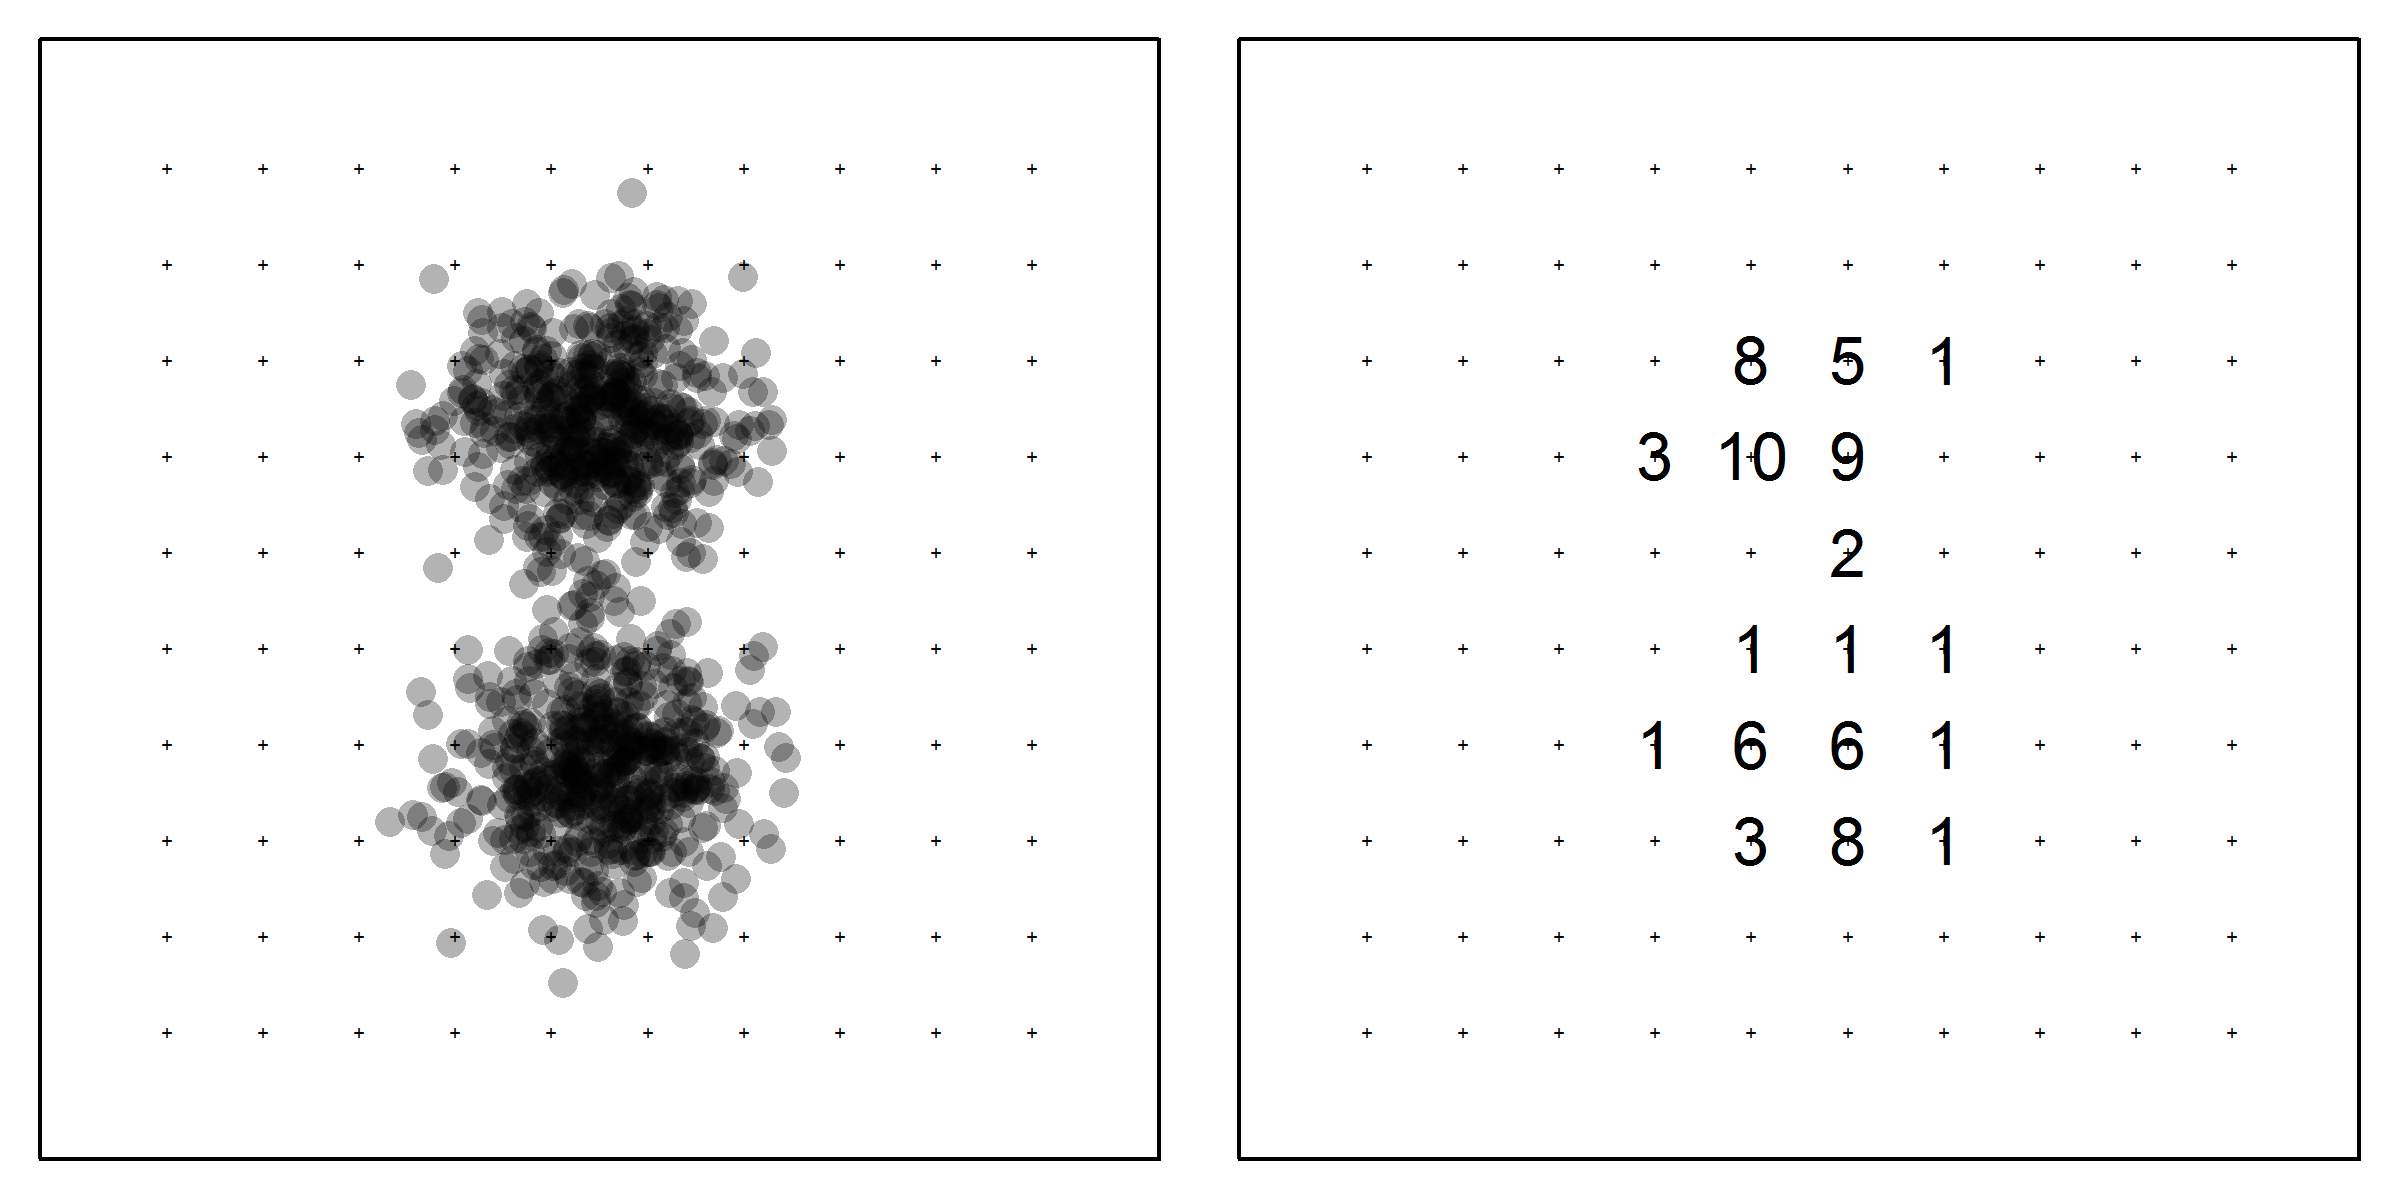
\includegraphics[width=0.5\textwidth]{Ch18-Unmarked/figs/heuristic}
\caption{Simulated count data at each of 100 camera traps
  (crosses) after $K=10$ sampling occasions. The black dots are the
  locations of two animal activity centers. The
  spatial count model estimates %attempts to estimate
  both the location and number of activity centers exposed to
  sampling using such spatially-referenced count data.}
\label{chapt-unmarked.fig.heur}
\end{figure}




\subsection{Types of spatial correlation}

The spatial correlation dealt with by the SC model is assumed to arise
from animal movement; however, this is just one type of spatial
correlation that may exist in ecological count data. Another common
type of spatial correlation results from the spatial correlation of
environmental covariates. Habitat variables, such as, the percent cover
of deciduous forest in North America, will often be patchy rather than randomly
distributed, and this can result in spatial correlation in abundance,
and hence in count data.  Often, this type of spatial correlation can
be dealt with by simply including the habitat covariate in the
model. For example, a simple, non-spatially-explicit
species distribution model with only a few habitat variables can result in a
distribution map that reflects the spatial correlation in abundance
\citep{sillett_etal:2012,royle_etal:2012mee2}.
The point is that the relevant assumption of non-spatial models (e.g. GLMs) is that
no spatial correlation exists in the \textit{residuals}, and often,
any spatial correlation apparent in the counts can be accounted for using
covariates. This may be obvious, but
it is a point that seems to be frequently misunderstood.

Of course, sometimes spatial correlation exists in residuals even
after including covariate effects. This may be due to
unobserved covariates or unobserved processes such as dispersal. When
mechanistic models cannot be developed to describe these processes,
several options exist for handling spatial correlation as a nuisance
\citep{besag_kooperber:1995,zuur_etal:2009,wikle:2010}.
In the context of SCR models, including the SC model dealt with in this
chapter, movement-induced spatial correlation is always explicitly
modeled, and other sources of spatial correlation can be accounted for
as well. For instance,
environmentally-induced spatial correlation can be modeled by adopting an
inhomogeneous point process model for the activity centers. That is,
the point process intensity can be modeled as a function of observed
covariates, and theoretically, it should be possible to allow for
spatially-correlated random effects to deal with unobserved covariates.
See Chapt.~\ref{chapt.state-space} for details.




\section{Spatial Count Model}

\subsection{Data}

Whereas traditional SCR models require spatially-referenced
individual encounter histories, the SC model requires simple
spatially-reference count data.
Let $n_{jk}$ be the count data at sampling location $j$
on occasion $k$. The entire $J \times K$ matrix of
counts will be denoted $\bf{n}$. A sampling location in this context
could be any device capable of recording count data, such as a
human observer or a camera trap, and
one of the benefits of the SC model is that it
can be applied to data collected using many different survey
methods. For ease of presentation, we will refer to sampling devices
as traps, but remember that a trap is just something capable of
recording count data. As in all SCR models, we also require the
coordinates of the $J$ traps, and we denote the location of trap $j$
by ${\bf x}_j$. In some instances, additional data might be available such as
trap-specific covariates, state-space covariates,
information on the identities of a subset of individuals, or perhaps
even distance data. We consider some of these model extensions in
Sec.~\ref{unmarked.sec.ext}, but for the time being we ignore these %extraneous
possibilities so that we can focus on the basic model.

\subsection{Model}

The state model is exactly the same as the one we have dealt with
throughout
this book. It is a point process describing the number and distribution of
activity centers in the state-space $\mathcal{S}$. Although it might
be possible to fit inhomogeneous point process models using the
methods described in Chapt.~\ref{chapt.state-space},
given the simplicity of the data, we concentrate on a homogeneous point process
$\{{\bf s}_i, \ldots, {\bf s}_N\} \sim \text{Uniform}(\mathcal{S})$
where ${\bf s}_i$ is the activity center of individual $i$ in the
population of size $N$. For the moment, we will assume that $N$ is
known.

The observation model is the same as in other SCR models %covered
in the sense that it describes the probability of encountering individual
$i$ at trap $j$, conditional on the location of the individual's
activity center. The specific encounter process will depend on the
sampling method, and here we consider the standard camera trapping
situation in which an individual can be encountered at multiple traps
during a single occasion, say one night during a camera-trapping
study, and it can be detected multiple times at a single trap during
an occasion. This is the Poisson encounter model (a.k.a. the count
detector case) described in Chapt.~\ref{chapt.poisson-mn}. Our
experience with alternative observation models such as the
Bernoulli and multinomial models
suggests that the parameters of the model may not be identifiable in
these cases, at least when no additional information is
available. This is a subject of ongoing research.

As before, we define $y_{ijk}$ as the
encounter data for individual $i$ at trap $j$ on occasion $k$, which
we model as:
\begin{equation}
 y_{ijk} \sim \mbox{Poisson}(\lambda_{ij})
\label{eq.latentPoisson}
\end{equation}
where $\lambda_{ij}$ is the encounter rate. A common encounter rate model is the
Gaussian, or half-normal, model:
\[
\lambda_{ij} = \lambda_0 \exp( - \| {\bf x}_j - {\bf s}_i \|^2 / 2\sigma^2)
\]
in which $\lambda_0$ is the baseline encounter rate,
$\| {\bf x}_j - {\bf s}_i \|$ is the Euclidean distance between the
trap and activity center, and $\sigma$ is the
scale parameter determining the degree to which encounter rate decreases with
distance. In this context, $\sigma$ also determines the amount of
correlation among the counts because if $\sigma$ is low relative to
the trap spacing, then it is unlikely that an individual will be
detected at multiple traps.

When individuals cannot be uniquely identified, the encounter histories cannot
be directly observed, which seems like a massively insurmountable
problem of epic proportions.
The solution of \citet{chandler_royle:2012} is the same one we routinely apply when we
cannot directly observe the process of interest -- we regard the
encounter histories as latent variables. This leaves the remaining
task of specifying the relationship between the count data and
the encounter histories, i.e. we need a model of $[{\bf n}|{\bf y}]$
where $\bf y$ represents the entire collection of encounter
histories. In this case, there is only one possibility because, by
definition, the count data are simply a
reduced-information summary of the latent encounter histories. That
is, they are the sample- and trap-specific totals, aggregated over all
individuals:
\begin{equation}
n_{jk} = \sum_{i=1}^{N} y_{ijk}.
\label{unmarked.eq.ny}
\end{equation}
So, unlike most model-development problems faced in this book, we
don't have to consider competing probability models for
$[{\bf n}|{\bf y}]$, but instead, we recognize the fact that the
relationship between the counts and the latent encounter histories is
deterministic. This deterministic constraint poses some computational
challenges, which we discuss below. But first we present some
alternative formulations of the model.

Recall from Chapt.~\ref{chapt.modeling} that the sum of two or more
Poisson random variables is also a Poisson random variable.
Specifically, if $x_1 \sim \text{Poisson}(\lambda_1)$ and
$x_2 \sim \text{Poisson}(\lambda_2)$, then $(x_1+x_2) \sim
\text{Poisson}(\lambda_1 + \lambda_2)$. Thus,
under this Poisson model for the latent encounter histories,
the count data can be modeled as Poisson:
\begin{equation}
n_{jk} \sim \mbox{Poisson}( \Lambda_{j} )
\label{eq:nagg}
\end{equation}
where
\[
 \Lambda_{j} = \lambda_0 \sum_{i} \exp(\| {\bf x}_j - {\bf s}_i \|^2 / 2\sigma^2),
\]
and because $\Lambda_j$ does not depend on $k$, we can
aggregate the replicated counts, defining
$n_{j.} = \sum_{k} n_{jk}$ and then
\[
 n_{j.} \sim \mbox{Poisson}( K \Lambda_{j} ).
\]
As such, $K$ and $\lambda_{0}$ serve equivalent roles as affecting
baseline encounter rate. Formulating the model in terms of the
aggregated count data demonstrates that the model can be
applied to data from a single sampling occasion ($J \equiv 1$) as has
been noted elsewhere for standard SCR models
\citep{efford_etal:2009ecol}. In the context of studying marked
populations, the model parameters will only be identifiable in the
$J\equiv 1$ case if an animal can be captured at multiple traps during
a single occasion. The SC model essentially requires the same thing,
which is to say that it requires correlation in the count data
resulting from an individual being captured in multiple,
closely-spaced traps.

This formulation of the model in terms of the aggregate count also
simplifies computations as the latent encounter histories
do not need to be updated in the MCMC estimation
scheme; however, retaining them in the formulation of the model
is important if some individuals are uniquely marked. This is because
uniquely identifiable individuals produce
observations of some of the $y_{ijk}$ variables, which we elaborate
on in the next chapter.





\subsection{On $N$ being unknown}
\label{unmarked.sec.N}

Even though there are no observed encounter histories in the situation
we consider here, we can still use data augmentation
\citep{tanner_wong:1987,liu_wu:1999} to resolve the
problem that $N$ is unknown. In fact, we are actually using two
different types of data augmentation since we first augment the
observed data with latent encounter histories, and then we augment
this latent data array with a set of all-zero encounter
histories. This approach turns out to be very similar to other data
augmentation schemes used to model spatial dependence in other contexts
\citep{wolpert_ickstadt:1998,best_etal:2000}.

Although the process of data augmentation should be familiar by now,
we briefly review the basics.
For homogeneous point process models, $N$ is typically modeled as
$N \sim \text{Binomial}(M, \psi)$, which is equivalent
to a discrete uniform prior on $N$ if $\psi \sim \text{Uniform}(0,1)$.
Since a binomial model is
equivalent to a series of $M$ independent Bernoulli trials, %hence
we can rewrite $N \sim \text{Binomial}(M, \psi)$ as $z_i \sim
\text{Bernoulli}(\psi)$ where $z_i$ is an auxiliary variable
indicating if individual $i$ is a member of the population, such that $N =
\sum_{i=1}^M z_i$. Having expanded the model to include a prior on $N$, we
can summarize the SC model, with a Gaussian observation model, as follows:
\begin{gather*}
  z_i \sim \text{Bernoulli}(\psi) \\
  y_{ijk} \sim \text{Poisson}(\lambda_{ijk} z_i) \\
  \lambda_{ijk} = \lambda_0\exp(-\|{\bf x}_j - {\bf s}_i\|^2)/(2\sigma^2) \\
  n_{jk} = \sum_{i=1}^M y_{ijk} %\\
\end{gather*}



\subsection{Inference}

Bayesian analysis can proceed once suitable priors have been put on
the hyperparameters $\psi$, $\sigma$, and
$\lambda_0$. \citet{chandler_royle:2012} provided \R~code for fitting
the model using MCMC, and they evaluated the model's performance with
uniform priors on the three hyperparameters. They also discussed the
possibilities and effects of including prior knowledge about $\sigma$
into the model. In Sec.~\ref{unmarked.sec.app}, we explain how the model can be
implemented using \jags, but first we briefly contemplate the viability of classical
analysis of this model.

The obvious challenge faced when conducting a classical analysis of
this model is that the number of latent variables in huge. In all SCR models, the activity centers are
latent, but now, even the encounter histories are latent.
Maximizing likelihoods with latent variables (random effects) involves
integrating (or summing) over all possible values of the latent
variables. For the activity centers, this is typically accomplished by
integrating the conditional-on-$\bf s$ likelihood $[{\bf y}_i|{\bf s}_i]$ over the two-dimensional
state-space $\mathcal{S}$ (Chapt.~\ref{chapt.mle}). However, with
the SC model, we have to sum
over all possible encounter histories %$\mathcal{H}$
meeting the constraint of Eq.~\ref{unmarked.eq.ny}. The
number of possible encounter histories
will, in general, be too high to make the likelihood tractable,
and thus we do not think that maximum likelihood is a viable option
for analyzing this model. However, one might be able to obtain
approximate maximum likelihood estimates using simulation-based methods
\citep{lele_etal:2010}, which will typically be more computationally
challenging than the Bayesian analysis.



\section{How Much Correlation Is Enough?}
In Chapt.~\ref{chapt.design}, we noted that if trap spacing is too
wide relative to the encounter rate parameter $\sigma$, then few
spatial recaptures will be realized and the model parameters will be
estimated poorly. The same principal applies here --
$\sigma$ shouldn't be too small or too large relative to trap
spacing or else the counts will be i.i.d. Poisson random variables. So
how much correlation is enough? Phrased differently, what is the ideal
ratio of $\sigma$ to trap spacing to ensure correlation and minimize
the variance of the posterior distributions? We see two options for
answering this questions, both of which are topics in need of
additional research. The first approach is to use the methods
described in Chapt.~\ref{chapt.design}, i.e. by either conducting
simulation studies with various trap spacing to $\sigma$ ratios, or to
analytically minimize a variance criterion for a given set of
sampling conditions and effort. The former approach was used by
\citet{chandler_royle:2012} whose limited simulation study indicated
that an ideal ratio is approximately 2. This agrees with
findings from previous research on the optimal design of SCR studies
(Chapt.~\ref{chapt.design}), as it should.

A second approach that may be of use if a data set has already been
collected is to use standard techniques from spatial statistics to
determine if adequate correlation exists in the counts. For example,
one might compute Ripley's $K$-statistic or generate (semi-)variograms
\citep{illian_etal:2008}. We have not studied the utility of such
approaches, but it seems worthy of investigation.



\section{Applications}
\label{unmarked.sec.app}

\subsection{Simulation example}

Simulating data under the SC model proceeds by first simulating
standard SCR encounter history data and then collapsing it into count
data. The following blocks of \R~code generate data from
the model, %shown in Sec.~\ref{unmarked.sec.N},
with parameters
$\sigma=5$, $\lambda_0=0.4$, and $N=50$. The state-space is a
$[0, 100] \times [0, 100]$ square, and a grid of 100 traps
is centered in the middle.
The first block of code generates the trap coordinates
$X$ and the $N=50$ activity centers:
\begin{small}
\begin{verbatim}
> tr <- seq(15, 85, length=10)
> X <- cbind(rep(tr, each=length(tr)),
+            rep(tr, times=length(tr)))    # 100 trap coords
> set.seed(10)
> xlim <- c(0, 100); ylim <- c(0, 100)     # S is [0,100]x[0,100] square
> A <- (xlim[2]-xlim[1])*(ylim[2]-ylim[1])/1e4 # Area of S
> mu <- 50                                 # Density (animals/unit area)
> N <- rpois(1, mu*A)                      # Generate N=50 as Poisson deviate
[1] 50
> s <- cbind(runif(N, xlim[1], xlim[2]), runif(N, ylim[1], ylim[2]))
\end{verbatim}
\end{small}
We could have set $N=50$ directly, but instead we treated density
as a fixed parameter ($\mu=50$) and generated $N$ as a random
variable -- it just so happens that with the specified random seed,
$N$ equals 50.

Now we can generate the encounter histories under the
Poisson observation model. Let's suppose that sampling is conducted
over $K=5$ nights.
\begin{small}
\begin{verbatim}
> sigma <- 5
> lam0 <- 0.4
> J <- nrow(X)
> K <- 5
> y <- array(NA, c(N, J, K))
> for(j in 1:J) {
+     dist <- sqrt((X[j,1]-s[,1])^2 + (X[j,2] - s[,2])^2)
+     lambda <- lam0*exp(-dist^2/(2*sigma^2))
+     for(k in 1:K) {
+         y[,j,k] <- rpois(N, lambda)
+     }
+ }
\end{verbatim}
\end{small}
The object \verb+y+ is the $N \times J \times K$ array of encounter
data, which cannot be directly observed if the animals are unmarked.
Converting the encounter data to count data can be accomplished using a single
\verb+apply+ command.
\begin{small}
\begin{verbatim}
> n <- apply(y, c(2,3), sum)
> dimnames(n) <- list(paste("trap", 1:J, sep=""),
+                     paste("night", 1:K, sep=""))
> n[1:4,]
      night1 night2 night3 night4 night5
trap1      1      0      0      0      0
trap2      1      2      2      0      1
trap3      1      0      0      1      0
trap4      0      0      0      0      0
\end{verbatim}
\end{small}
This displays the first 4 rows of \verb+n+, the $J \times K$
matrix of counts.


The question now is: Is it possible to estimate the parameters? In our
simulated dataset we have $J \times K = 500$ data points, but how many
parameters do we need to estimate?
A frequentist might say that there are only 3 parameters: $\lambda_0$,
$\sigma$, and $N$ (or density $\mu$) because inference about the
latent parameters is carried out using prediction methods after the 3
hyperparameters have been estimated. However, a Bayesian would
probably say that each $\bf s$ and each element of the latent
encounter array $\bf y$ is a parameter in need of a posterior. From
this perspective there are far more parameters than data points, and
thus it would appear as though the situation is dire. Whether or not
the parameters are actually estimable is a rather difficult question
to answer. One simplistic, but not definitive, approach for addressing
the question is to conduct a simulation study and evaluate the
frequentist performance of the model by asking how often the
data-generating values are included in confidence/credible intervals,
and how biased are point estimates. \citet{chandler_royle:2012}
conducted such a simulation study and found that, while the variance
of the posterior distribution was high by most standards, the bias of
the posterior mode of $N$ was small and the coverage of the credible
intervals was close to nominal. Moreover, they found no evidence that the
posterior distributions were dominated by the priors, further
supporting the conclusion that spatial correlation in the count data
is sufficient for estimating density and encounter probability
parameters.

At this point in time the SC model can only be fit using one of the
\bugs~engines, or using custom software like the \R~code accompanying
\citet{chandler_royle:2012}. Although \bugs~might provide the most
flexible option for fitting the model, it is not
straight-forward because of the
constraints in the model. In \textbf{WinBUGS}, the
$n_{jk} = \sum_i y_{ijk}$
constraint can be
enforced using the so-called ``ones-trick'', but we prefer
\jags~because it has a distribution
called \verb+dsum+ that was designed for this type
of situation in which the observed data are a sum of random
variables. Panel~\ref{unmarked.panel.jags1} shows the \jags~code, but
we abbreviated the
arguments to \verb+dsum+ because in practice you need to provide all $M$ of
them. The code looks slightly unwieldy if $M$ is large, but you can easily create
it using the \verb+paste+ function in \R. Here is an example, with an
unrealistically small value of $M=10$:
\begin{small}
\begin{verbatim}
> paste("y[", 1:10, ",j,k]", sep="", collapse=", ")
[1] "y[1,j,k], y[2,j,k], y[3,j,k], y[4,j,k], y[5,j,k], y[6,j,k],
y[7,j,k], y[8,j,k], y[9,j,k], y[10,j,k]"
\end{verbatim}
\end{small}


\begin{panel}[ht]
\centering
\rule[0.05in]{\textwidth}{.03in}
\begin{small}
\begin{verbatim}
model{
sigma ~ dunif(0, 200) # Tailor this to your state-space
lam0 ~ dunif(0, 5)    # consider dgamma() as an alternative
psi ~ dbeta(1,1)
for(i in 1:M) {
   z[i] ~ dbern(psi)
   s[i,1] ~ dunif(xlim[1], xlim[2])
   s[i,2] ~ dunif(ylim[1], ylim[2])
   for(j in 1:J) { # Number of traps
       distsq[i,j] <- (s[i,1] - X[j,1])^2 + (s[i,2] - X[j,2])^2
       lam[i,j] <- lam0 * exp(-distsq[i,j] / (2*sigma^2))
       for(k in 1:K) { # Number of occasions
           y[i,j,k] ~ dpois(lam[i,j]*z[i])
           }
       }
   }
for(j in 1:J) {
   for(k in 1:K) {
       n[j,k] ~ dsum(y[1,j,k], y[2,j,k], ..., y[200,j,k])
       }
   }
N <- sum(z[])   # Realized population size
A <- (xlim[2]-xlim[1])*(ylim[2]-ylim[1]) # Area of state-space
D <- N / A      # Realized density
ED <- (M*psi)/A # Expected density
}
\end{verbatim}
\end{small}
\rule[0.15in]{\textwidth}{.03in}
\caption{\jags~code defining the spatial count model. This version
  includes the latent encounter histories. Note the abbreviated
  arguments to dsum().}
\label{unmarked.panel.jags1}
\end{panel}


The \jags~model in Panel~\ref{unmarked.panel.jags1} can be used to
fit the version of the model in which the latent encounters are
updated at each Monte Carlo iteration. One challenge faced when using
this version of the model is that \jags~cannot auto-generate initial values
that honor the constraints in the model, so it is necessary to provide
them. The following code presents one fairly general way of creating
acceptable starting values and formatting the data for analysis using
the \texttt{rjags} package:
\begin{small}
\begin{verbatim}
> library(rjags)
> dat1 <- list(n=n, X=X, J=J, K=K, M=200, xlim=xlim, ylim=ylim)
> init1 <- function() {
+    yi <- array(0, c(dat1$M, dat1$J, dat1$K))
+    for(j in 1:dat1$J) {
+         for(k in 1:dat1$K) {
+            yi[sample(1:dat1$M, dat1$n[j,k]),j,k] <- 1
+        }
+    }
+    list(sigma=runif(1, 1, 2), lam0=runif(1),
+         y=yi, z=rep(1, dat1$M))
+ }
> pars1 <- c("lam0", "sigma", "N", "mu")
\end{verbatim}
\end{small}

The code in Panel~\ref{unmarked.panel.jags1} is useful because it shows how
closely this model is related to standard SCR models, and it provides
the basis for including data on both marked and unmarked individuals,
as will be discussed in the next chapter. However, this model runs
very slowly, even when using a fast 64-bit machine with chains run in parallel. The code
in Panel~\ref{unmarked.panel.jags2} runs much faster because it
does not include the latent encounter histories.

\begin{panel}[ht]
\centering
\rule[0.05in]{\textwidth}{.03in}
\begin{small}
\begin{verbatim}
model{
sigma ~ dunif(0, 200)
lam0 ~ dunif(0, 5)
psi ~ dbeta(1,1)
for(i in 1:M) {
   z[i] ~ dbern(psi)
   s[i,1] ~ dunif(xlim[1], xlim[2])
   s[i,2] ~ dunif(ylim[1], ylim[2])
   for(j in 1:J) { # Number of traps
       distsq[i,j] <- (s[i,1] - X[j,1])^2 + (s[i,2] - X[j,2])^2
       lam[i,j] <- lam0 * exp(-distsq[i,j] / (2*sigma^2)) * z[i]
       }
   }
for(j in 1:J) {
   bigLambda[j] <- sum(lam[,j])
   for(k in 1:K) {
       n[j,k] ~ dpois(bigLambda[j])
       }
   }
N <- sum(z[])
}
\end{verbatim}
\end{small}
\rule[0.15in]{\textwidth}{.03in}
\caption{\jags~code defining the spatial count model. This version
  does not include the latent encounter histories, and thus runs much
  faster than the code in Panel~\ref{unmarked.panel.jags1}.}
\label{unmarked.panel.jags2}
\end{panel}



An even faster (but perhaps less efficient) alternative is to use the
\verb+scrUN+ function in \texttt{scrbook}.
The usage is as follows:
\begin{small}
\begin{verbatim}
> out1 <- scrUN(n=n, X=X, M=300, niter=25000, xlims=xlim, ylims=ylim,
               inits=list(lam0=0.3, sigma=rnorm(1, 5, 0.1)), updateY=TRUE,
               tune=c(0.004, 0.09, 0.35))
\end{verbatim}
\end{small}
where \verb+n+ is the matrix of counts, \verb+X+ is the trap
coordinate matrix, \verb+M+ sets the size of the data-augmented latent
data, \verb+xlims+ and \verb+ylims+ define the
rectangular state-space, \verb+inits+ is a list of starting values,
and \verb+updateY+ determines if the latent encounter histories are
updated as part of the MCMC algorithm. In general, we recommend using the option
\verb+updateY=FALSE+ because the Markov chains tend to mix
better. Even so, it can be important to fiddle with the tuning parameters until the
acceptance rates are between 40--60\%. Otherwise, the Markov chains
will exhibit extremely high autocorrelation. This is one reason to favor
\jags~over our implementation in \texttt{scrbook} since \jags~finds
suitable tuning parameters automatically during the adaptive phase
(when using Metropolis updates).

We fit the model to the simulated data using both formulations -- with and without
the latent encounter histories -- using both \jags~and \verb+scrUN+.
Table~\ref{unmarked.tab.sim} shows summaries of 25000 posterior draws,
and suggests that while the true parameter values are easily covered
by the 95\% credible intervals, the intervals are rather wide. This
low precision is not just a peculiarity of this particular data set --
it will generally be low unless the sample size is very large,
as noted by \citet{chandler_royle:2012}. Furthermore,
autocorrelation of the samples will typically be high
Fig.~\ref{unmarked.fig.Nsim},
and thus it may take many iterations to achieve convergence.
The results shown in Fig.~\ref{unmarked.fig.Nsim} also indicate that
the algorithm that includes the latent encounter histories
seems to have a hard time exploring the region of the posterior in
which $N$ is low. Given these technical difficulties, we recommend
using the \jags~implementation (based on
Panel~\ref{unmarked.panel.jags2}), and it is always a good idea to use
MCMC diagnostic tools such as those available in the \texttt{coda}
package (Chapt.~\ref{chapt.mcmc}).

\begin{table}
  \centering
  \caption{Posterior summaries from the spatial count (``SC'') model
    applied to simulated data using \texttt{scrbook} and \jags. 25000
    samples were generated, but substantial Monte Carlo error is still
    evident. All parameters were given uniform priors.}
  \begin{tabular}{lrrrrr}
    \hline
    Parameter        & Mean   & SD     & 2.5\%  & 50\%   & 97.5\%  \\
    \hline
    \multicolumn{6}{c}{\tt scrUN(..., updateY=FALSE)}              \\
    $\sigma=5$         & 4.718  & 0.922  & 3.239  & 4.615  & 6.833   \\
    $\lambda_0=0.4$      & 0.500  & 0.136  & 0.268  & 0.489  & 0.793   \\
    $N=50$              & 60.653 & 31.067 & 21.000 & 54.000 & 137.000 \\
    \hline
    \multicolumn{6}{c}{\tt scrUN(..., updateY=TRUE)}               \\
    $\sigma$         & 4.554  & 0.784  & 3.216  & 4.486  & 6.264   \\
    $\lambda_0$      & 0.489  & 0.131  & 0.262  & 0.479  & 0.775   \\
    $N$              & 64.772 & 30.162 & 26.000 & 59.000 & 140.000 \\
    \hline
    \multicolumn{6}{c}{\jags~(without latent encounter histories)} \\
    $\sigma$         & 4.70   & 0.88   & 3.24   & 4.66   & 6.63    \\
    $\lambda_0$      & 0.52   & 0.14   & 0.27   & 0.52   & 0.80    \\
    $N$              & 58.55  & 30.30  & 20.00  & 52.00  & 135.00  \\
    \hline
  \end{tabular}
  \label{unmarked.tab.sim}
\end{table}


\begin{figure}
  \centering
  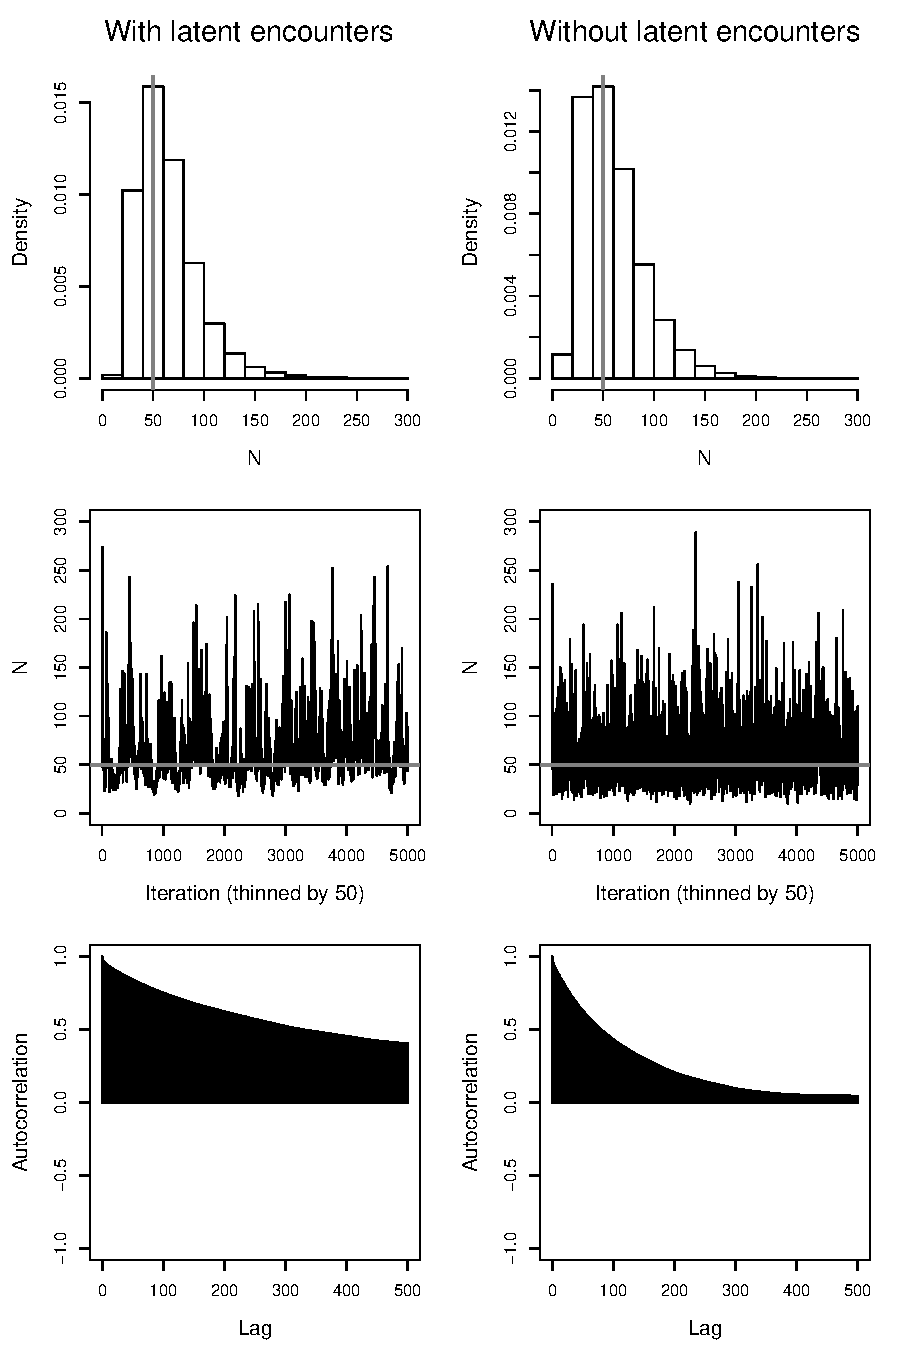
\includegraphics[width=0.8\textwidth]{Ch18-Unmarked/figs/mc1mc2}
  \caption{MCMC results for the parameter $N$ from the two algorithms
    (with and without the latent encounter histories). The first
    row contains the histograms of the posterior distributions, the second row
    contains the history (or trace) plots, the third row shows the
    autocorrelation plots.}
  \label{unmarked.fig.Nsim}
\end{figure}

The take-home message is that, even with simulated data,
the precision of the posterior distributions is
low and mixing is poor. This should be expected given that we are
asking so much from so little data. In essence, we are trying to fit a
point process model while being twice removed from the actual point
(activity center) locations. These difficulties may warrant the investigation of simpler
models at the expense of the mechanistic description of the system. Another option is to
figure out ways of improving model precision -- options we discuss in
Sec.~\ref{unmarked.sec.ext}. Before doing so, we re-analyze the
Northern Parula ({\it Parula americana}) data
described in \citet{chandler_royle:2012}



\subsection{Northern parula in Maryland}

The parula data are standard avian point count data, with one
exception. Typically, when studying
passerines, points are spaced by $>200$ m in order to maintain
statistical independence. In contrast,
the parula data were collected at
105 points located on a 50-m grid, which virtually ensures spatial
correlation since the parula song can be heard from distances $>$50 m.
Each point was surveyed 3 times during June 2006, and
Fig.~\ref{fig:nopaDat} depicts the resulting spatially-correlated
counts ($n_{j.}$). A total of 226 detections were made with a maximum
count of 4 during a single survey. At 38 points, no birds were
detected. All but one of the detections were of singing males, and
this one observation was not included in the analysis.

\begin{figure}
  \centering
  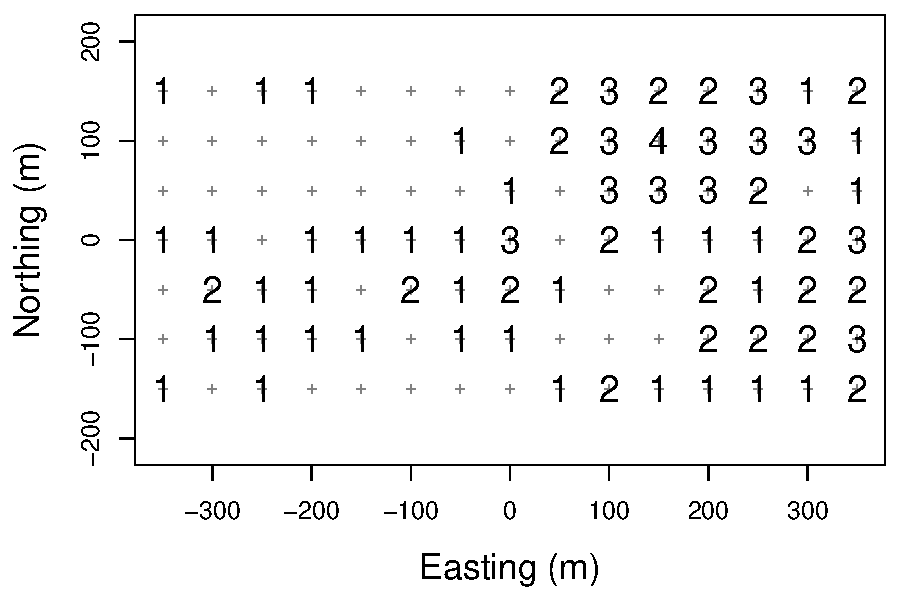
\includegraphics[width=0.8\textwidth]{Ch18-Unmarked/figs/nopaCounts}
  \caption{Spatially-correlated counts of northern parula. Gray
    crosses are the locations of the 105 point count
    stations. Superimposed are the number of detections after 3 survey occasions.}
  \label{fig:nopaDat}
\end{figure}

We fit the model using \jags~and the code from
Panel~\ref{unmarked.panel.jags2}, which does not include the latent
encounter histories. For comparative purposes, we used two sets of priors:
(1) the improper uniform priors considered by
\citet{chandler_royle:2012} and (2) proper $\text{Gamma}(0.001,0.001)$
priors for $\sigma$ and $\lambda_0$ as well as an approximate
$N \propto 1/N$ prior, which is (almost) the Jeffreys prior (see
\citet{link:2013} and \citet{link_barker:2010} for details on Jeffreys
prior). The state-space created by buffering the grid of point count
locations by 250 m. $M$ was set to 300. To reduce computation time, we
used the \texttt{parallel} package and distributed 3 chains to 3
separate cores. The entire example can be reproduced using the code on
the help page for \verb+nopa+ in our \R~package \texttt{scrbook}. The
following code illustrates the essential elements:
\begin{small}
\begin{verbatim}
> library(scrbook)
> library(rjags)
> dat2 <- list(n = nopa$n, X = nopa$X, M=300, J=nrow(nopa$n), K=ncol(nopa$n),
+             xlim=c(-600, 600), ylim=c(-400, 400))
> init2 <- function() {
+    list(sigma=rnorm(1, 100), lam0=runif(1), z=rep(1, dat2$M))
+ }
> cl2 <- makeCluster(3) # Open 3 parallel R instances
> clusterExport(cl2, c("dat2", "init2", "pars1")) # send objects to 3 cores
> out2 <- clusterEvalQ(cl2, { # executes the folowing command on each core
+    library(rjags)
+    jm <- jags.model("nopa2.jag", dat2, init2, n.chains=1, n.adapt=1000)
+    jc <- coda.samples(jm, pars1, n.iter=150000)
+    return(as.mcmc(jc))
+ })
> mc2 <- mcmc.list(out2) # put the 3 chains together
> plot(mc2)
> summary(mc2)
\end{verbatim}
\end{small}



\begin{table}%[t]
  \centering
  \caption{Posterior summary statistics for spatial count
    model applied to the northern parula data. Note the sensitivity to
    the two sets of priors. }
  \begin{tabular}{llrrrrr}
    \hline
    Par         & Prior                       & Mean    & SD      & 2.5\%  & 50\%    & 97.5\%  \\
    \hline
    $N$         & $\text{DUnif}(0,300)$       & 38.474  & 37.275  & 1.000  & 29.000  & 138.000 \\
    $\lambda_0$ & $\text{Unif}(0,\infty)$     & 0.310   & 0.183   & 0.082  & 0.269   & 0.817   \\
    $\sigma$    & $\text{Unif}(0,\infty)$     & 127.935 & 99.303  & 44.760 & 87.291  & 438.374 \\
    \hline
    $N$         & $\propto 1/N$               & 29.591  & 32.555  & 1.000  & 19.000  & 119.000 \\
    $\lambda_0$ & $\text{Gamma}(0.001,0.001)$ & 0.309   & 0.194   & 0.078  & 0.261   & 0.843   \\
    $\sigma$    & $\text{Gamma}(0.001,0.001)$ & 150.183 & 105.044 & 48.735 & 117.069 & 447.616 \\
    \hline
  \end{tabular}
  \label{unmarked.tab.nopa}
\end{table}



\section{Extensions of the Spatial Count Model}
\label{unmarked.sec.ext}

\subsection{Improving Precision}

The results of the parula analysis are presented in
(Table~\ref{unmarked.tab.nopa}).
Once again, we see wide credible intervals for $N$, and also high
sensitivity to the priors. These limitations support the conclusions
of \citet{chandler_royle:2012} that researchers should: (1) elicit prior
information from the published literature and/or (2) mark a subset of
individuals when applying the SC model. Both of these options should
be readily accomplished in many studies, especially the first option
because extensive information on home range size has
been compiled for many species in diverse habitats
\citep[e.g.][]{degraaf_yamasaki:2001}, which can be
embodied as a prior distribution for the
encounter rate parameter $\sigma$ in a Bayesian
analysis (\citet{chandler_royle:2012}, Chapt.~\ref{chapt.scr0}).


In some cases, it may not be possible to mark any individuals, and no
prior information may exist about encounter parameters; however, it
may be possible to improve precision %of estimates
by collecting
auxiliary data, such as distance
measurements. In fact, in the parula study, detections were classified
as either within or beyond 150 m, and it seems sensible to expand the
model to accommodate this rudimentary distance sampling data.
But if auxiliary data such as distance measurements exist, why
bother with the SC model at all since density can be estimated using
the distance data alone? This is a good point, and in general, the
simplest model that does the job should be preferred.
The reasons why one might prefer an expanded SC model over a simple
distance sampling model include the ability to model spatial
correlation and the ability to model movement. But how exactly can the
SC model be extended to accommodate such auxiliary data?


The basic extension that we consider here is to use a type of
search-encounter model (Chapt.~\ref{chapt.search-encounter}) that
includes the activity centers ($\bf s$) and the
actual locations of individuals ($\bf u$).
By including both activity centers and actual locations
in the model, abundance in any region $\mathcal{B}$ is given by
\begin{equation}
N(\mathcal{B}) = \sum_i I({\bf u}_i \in \mathcal{B}).
\label{unmarked.eq.B}
\end{equation}
Thus, in the context of distance sampling studies in which the
distance data are recorded in discrete intervals, the region
$\mathcal{B}$ would be the area corresponding to a particular distance
interval. The probability of detecting the individuals
$N(\mathcal{B})$ would be the average detection probability $\bar{p}$,
which is computed by integrating a distance-based detection function
over the distance interval.

In other contexts, such as when conducting removal surveys, the region
$\mathcal{B}$ could be a fixed-area plot, such as a stream
segment. Again, Eq.~\ref{unmarked.eq.B} could be used to model local
abundance ($N(\mathcal{B})$), and detection probability within the region could be
modeled conditional on $N(\mathcal{B})$. A reasonably general
description of this model is as follows:
\begin{gather*}
  {\bf s}_i \sim \text{Uniform}(\mathcal{S}) \\
  {\bf u}_{ik} \sim \text{BVN}({\bf s}_i, {\bm \Sigma}) \\
  N(\mathcal{B}_{jk}) = \sum_{i=1}^M I({\bf u}_{ik} \in \mathcal{B}_{jk}) \\
  n_{jkl} \sim \text{Binomial}(N(\mathcal{B}_{jkl}), p)
\end{gather*}
where ${\bm \Sigma} = \begin{pmatrix} \tau & 0 \\ 0 &
  \tau \end{pmatrix}$, with $\tau$ governing the size of the bivariate
normal home range.
The interpretation of the parameter $p$ will depend upon the
survey protocol \citep{nichols_etal:2009}.

When plots are far enough apart that
individuals cannot move between them, the counts will be uncorrelated
and the model can be approximated using a non-spatial $N$-mixture model
allowing for temporary emigration \citep{chandler_etal:2011}.
In the next example, we consider data in which the plots are obviously
not independent.


\subsection{Dusky Salamanders in Maryland}

The independence assumption of the \citet{chandler_etal:2011} model
will not always hold. A prime example is in studies of aquatic
species in stream networks. For example, consider the data depicted in
Fig.~\ref{unmarked.fig.salct}. The figure shows counts of northern
dusky salamanders (\textit{Desmognathus fuscus}) in 25-m stretches on
a small stream in the Chesapeake and Ohio National Historic Park. The
data were collected by E.H.C. Grant and colleagues with the objective
of understanding the spatial and temporal dynamics of salamander
populations in response to seasonal and annual variations in stream
hydrology. More details the study can be found in \citet{grant_etal:2010}.

To sample the population, the stream networks were divided into 25-m
stretches, and in each stretch, ``temporary'' removal sampling was
conducted, which involves capturing and removing salamanders on 3
consecutive passes. The salamanders are placed in a bucket of water
for the brief 10-20 min duration of sampling, and then they are
released at the location of capture. The entire process is repeated
3-4 times per season (May-Aug). In a subset of streams and years,
individuals are marked, but in general it is too expensive to mark the
entire population, and the data considered here consists entirely of
unmarked individuals.

\begin{figure}
  \centering
  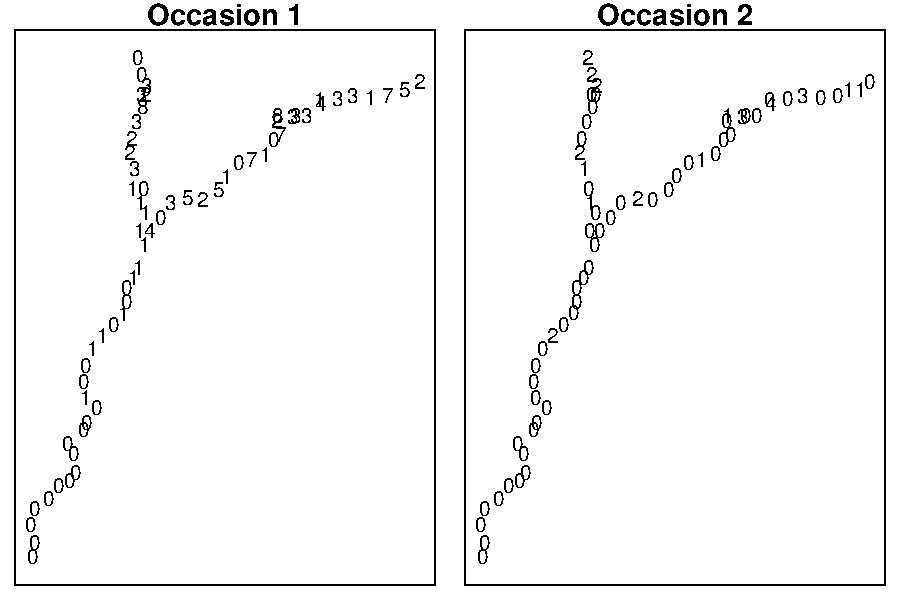
\includegraphics[width=0.8\textwidth]{Ch18-Unmarked/figs/saln27}
  \caption{Stream segment counts of northern dusky salamanders
    in the Chesapeake and Ohio National Historic Park,
    VA/MD. Each number is the count associated with a 25-m stretch in which 3 removal passes
    were made on 3 occasions each summer (only 2 occasions are shown
    here). Notice the consistency of the spatial correlation between
    occasions and the temporal decline in the counts.}
  \label{unmarked.fig.salct}
\end{figure}


The sampling protocol may be
thought of as a ``robust design'' \citep{pollock:1982}, with
``occasions'' (typically 1 day) being the primary period, and
secondary samples being the removal passes within the primary
periods. An obvious feature of these data is that the neighboring
counts are spatially correlated. In this case, we have reason to
believe that this correlation is the result of habitat preferences,
with individuals actively selecting habitat in the upper reaches of
the streams. This could be modeled as a function of a covariate
describing the distance from the mouth of the stream. Another obvious
feature of this data is that the pattern of spatial correlation
remains consistent between occasions, but the overall counts decline
markedly over the course of the season.
These phenomena can be explained by the fact that the salamanders have
relatively small home ranges, and this results in the consistent pattern of
correlation  among occasions. Furthermore, as the season progresses, the
streams dry out, and many individuals move underground.

Given the importance of movement within home ranges, which determines
the correlation among occasions, and movement underground, which
results in a decreasing number of individuals being available for
sampling, it would be helpful to have a model that describes both
processes and allows for evaluation of hypotheses regarding the
effects of environmental variables. For example, one might ask how
stream flow is related to the probability that an individual remains
active, i.e. aboveground.
A model describing this process could be used to predict
activity levels under future conditions. Although we do not
investigate covariate effects in this section, we do present a general
model allowing for movement among occasions, and for decreasing
availability over the season.

This expanded model is founded on the one described in the previous
section, but it also includes a removal model for the observation
process, and it includes a basic ``open'' population model to allow
for a decline in abundance over time
(Chapt.~\ref{chapt.open}). Actually, the population is not thought to
decline substantially during the season, but rather, the
number of individuals \textit{available} for detection declines
because many individuals move underground as the streams dry. Each of
these components is included in the \bugs~description of the
model presented in Panel~\ref{unmarked.panel.sal}.


\begin{panel}[ht]
\centering
\rule[0.05in]{\textwidth}{.03in}
\begin{small}
\begin{verbatim}
model {
phi ~ dbeta(1,1)      # "availability" parameter
tau ~ dunif(0, 1000)  # "movement parameter" of Gaussian kernel model
p ~ dbeta(1,1)        # detection prob
psi ~ dbeta(1,1)      # data augmentation parameter
for(i in 1:M) {
  z[i,1] ~ dbern(psi)        # is the individual real?
  z[i,2] ~ dbern(z[i,1]*phi) # and still aboveground?
  z[i,3] ~ dbern(z[i,2]*phi) # ...
  s[i] ~ dcat(PrSeg[]) # location (stream segment) of activity center
  for(g in 1:G) {
    PrU[i,g] <- exp(-distmat[s[i],g]^2/(2*tau^2)) # Pr(u | s)
    }
  for(k in 1:K) {
    u[i,k] ~ dcat(PrU[i,]) # location of guy i at time k
    for(g in 1:G) {
      y[i,g,k] <- (u[i,k] == g)*z[i,k] # was individual at u==g?
      }
    }
  }
for(j in 1:J) {
  for(k in 1:K) {
    NB[j,k] <- sum(y[,seg[j],k]) # Number in seg j at time k
    # removal model:
    n[j,1,k] ~ dbin(p, NB[j,k])
    NB2[j,k] <- NB[j,k] - n[j,1,k]
    n[j,2,k] ~ dbin(p, NB2[j,k])
    NB3[j,k] <- NB2[j,k] - n[j,2,k]
    n[j,3,k] ~ dbin(p, NB3[j,k])
    }
  }
N[1] <- sum(z[,1]) # Total abundance, occasion 1
N[2] <- sum(z[,2]) # Total abundance, occasion 2
N[3] <- sum(z[,3]) # Total abundance, occasion 3
}
\end{verbatim}
\end{small}
\rule[0.05in]{\textwidth}{.03in}
\caption{\bugs~description of model for the data shown in
  Fig.~\ref{unmarked.fig.salct}. The model allows for
  spatially-explicit temporary emigration, and for a decrease in
  abundance as individuals move underground throughout the course of
  the season.}
\label{unmarked.panel.sal}
\end{panel}

We fit this model to the data and obtained the posterior distributions
summarized in Table~\ref{unmarked.tab.dusky}. The results indicate that
the population size available for detection did decrease
rapidly during the season, the rate of which is determined by the
$\phi$ parameter. Modeling this parameter as a function of water flow
or volume would allow one to predict salamander activity under future
environmental conditions.
Another result of the analysis is that the movement parameter, $\tau$,
was relatively low, indicating that adult salamanders rarely move more
than 100 m from their home range center during a season. This explains
why the distribution of individuals within the stream remains
relatively constant over time. %Including this parameter in the model

\begin{table}
  \centering
  \caption{Posterior summarizes from removal model of salamander
    counts allowing for movement and decreasing population size over
    the course of a breeding season.}
  \begin{tabular}{lrrrrr}
    \hline
    Parameter & Mean    & SD     & 2.5\%   & 50\%    & 97.5\%  \\
    \hline
    $N_1$     & 178.393 & 16.346 & 151.000 & 177.000 & 214.000 \\
    $N_2$     & 62.322  & 6.884  & 51.000  & 62.000  & 77.000  \\
    $N_3$     & 21.202  & 3.695  & 15.000  & 21.000  & 29.000  \\
    $\phi$    & 0.348   & 0.038  & 0.275   & 0.348   & 0.425   \\
    $\tau$    & 27.427  & 3.200  & 21.293  & 27.173  & 33.706  \\
    $p$       & 0.396   & 0.053  & 0.294   & 0.394   & 0.502   \\
    \hline
  \end{tabular}
  \label{unmarked.tab.dusky}
\end{table}





\section{Summary and Outlook}

Unlike traditional models of count data used in ecology, the SC model
is parameterized in terms of \textit{individuals} -- individuals that just so
happen not to be marked. Although developing the model in terms of
latent encounters increases model complexity, several reasons exist for
accommodating this latent structure. First, it allows for
individual-level covariates, including the location of each individual
in the population. Second, by including an
underlying point process specific to individual activity centers (and
possibly locations in time), the model allows for modeling continuous
variation in density, which may result in bias when ignored in
conventional models of count data. Third, accommodating the
latent structure provides a more mechanistic description
of ecological systems, for example by attaching a
mechanism (movement) to the widely observed phenomenon of spatial
correlation in count data.

The SC model is a conceptually simple extension of standard SCR
models, but in terms of computational requirements and latent
structure, it is perhaps at the extreme end of what is possible to do
with count data. As is always true, the harder we try to mirror
reality with our models, the harder it becomes to estimate the
parameters of the system. In this chapter, we tried to emphasize that
as conceptually appealing as the SC model may be, it is unlikely to
produce satisfying results in the absence of additional
information. However, additional information such as home range size
estimates will often be available
for many species, and if not, we have provided an alternative method of
accommodating additional data in the form of distance measurements or
removal counts. This can greatly increase precision of estimates from studies
designed to make spatially-explicit inferences about population
processes.

Although we focused on the situation in which all individuals are
unmarked, one of the reasons for developing this class of models was to handle
the problem of estimating population size or density when only a
subset of individuals are marked. This topic is the subject of the
next chapter, which builds on a rich literature of combining data from
marked and unmarked individuals for purposes of designing efficient
studies \cite{bartmann_etal:1987,neal_etal:1993,conroy_etal:2008,mcclintock_white:2009}.



